\chapter{\ifproject%
\ifenglish Project Structure and Methodology\else โครงสร้างและขั้นตอนการทำงาน\fi
\else%
\ifenglish Project Structure\else โครงสร้างของโครงงาน\fi
\fi
}

\makeatletter

% \renewcommand\section{\@startsection {section}{1}{\z@}%
%                                    {13.5ex \@plus -1ex \@minus -.2ex}%
%                                    {2.3ex \@plus.2ex}%
%                                    {\normalfont\large\bfseries}}

\makeatother
%\vspace{2ex}
% \titleformat{\section}{\normalfont\bfseries}{\thesection}{1em}{}
% \titlespacing*{\section}{0pt}{10ex}{0pt}

\section{โครงสร้างโดยรวมของโครงงาน (Project Overview) }
\begin{mypara}
    \indent โครงงานนี้เป็นระบบสนับสนุนการตัดสินใจสำหรับการวางแผนระบบขนส่งสาธารณะ 
    โดยจะจัดทำเป็นเว็บแอพลิเคชั่นสำหรับการจำลอง และมีการสรุปผลลัพธ์ที่ได้จากการจำลองในรูปแบบทางสถิติ
    ซึ่งในการทำงานของระบบนี้จะมี 4 องค์ประกอบหลักดังนี้  
\end{mypara}


\begin{figure}[H]
    \centering
    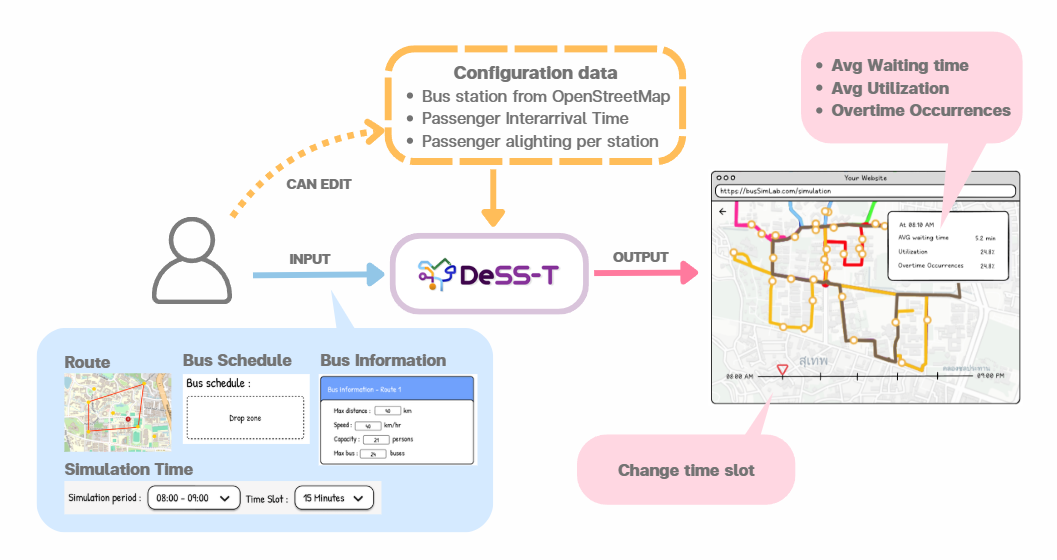
\includegraphics[width=\textwidth,height=0.9\textheight,keepaspectratio]{overview.png}
    \caption{แผนภาพโดยรวมของโครงงาน}
    \label{fig:overview}
\end{figure}

\subsection{Input data (Scenario data)}
\begin{mypara}
  \indent เป็นข้อมูลที่ผู้ใช้สามารถปรับเปลี่ยนพารามิเตอร์ได้บ่อย ๆ เพื่อจำลองสถานการณ์ต่าง ๆ 
  สำหรับการเปรียบเทียบและวางแผน ประกอบด้วย เส้นทางการให้บริการของรถในแต่ละสายบริการ 
  ตารางเวลาการออกรถ ช่วงเวลาที่ต้องการดูผลการจําลอง ข้อมูลของรถซึ่งมี 
  ความจุผู้โดยสารระยะทางที่สามารถวิ่งได้สูงสุด ความเร็วในการวิ่ง
\end{mypara}
\subsection{Configuration data (Base data)}
\begin{mypara}
  \indent เป็นส่วนของข้อมูลที่ใช้เป็นพื้นฐานในการจำลองซึ่งจะไม่ค่อยมีการเปลี่ยนแปลงบ่อย 
  ได้แก่ ข้อมูลช่วงระยะห่างของเวลาที่ผู้โดยสารแต่ละคนมาถึงที่สถานี ข้อมูลของจำนวนผู้โดยสารที่ลงจากรถในแต่ละสถานี 
  และข้อมูลที่เกี่ยวข้องกับสถานีซึ่งจะเก็บในรูปแบบของ network model ซึ่งจะมี 
  node เป็นรายชื่อสถานี และ มี edge เป็นระยะทางละหว่างแต่ละสถานี
  \end{mypara}
\subsection{Simulation Engine}
\begin{mypara}
  \indent เป็นส่วนที่ทำหน้าที่ในการจำลองระบบขนส่งสาธารณะตามข้อมูลที่ได้รับจากส่วน input 
  และ configuration data ซึ่งจะใช้เทคนิคการจำลองแบบเหตุการณ์ไม่ต่อเนื่อง (discrete-event simulation) 
  ในการจำลองระบบขนส่งสาธารณะ 
\end{mypara}
\subsection{Output}
\begin{mypara}
  \indent เป็นส่วนที่แสดงผลลัพธ์ที่ได้จากการจำลอง โดยจะมีข้อมูล การรอเฉลี่ยของผู้โดยสาร อัตราการใช้งานของรถ 
  และอัตราการเกิดเหตุการณ์ที่รถบัสมีการใช้งานเกินเวลาหรือระยะทางที่กำหนด
  ซึ่งจะมีข้อมูลแสดงทั้งข้อมูลรวมทุกสถานี และข้อมูลรายละเอียดของแต่ละสถานีแยกกัน รวมถึงจะมี dashboard 
  สำหรับแสดงผลลัพธ์ในรูปแบบกราฟเพื่อให้ผู้ใช้สามารถวิเคราะห์ข้อมูลได้ง่ายขึ้น
\end{mypara}
\section{ ขั้นตอนการทำงาน (Process Overview)}
\begin{mypara}
    \indent โครงงานนี้ทำงานโดยนำข้อมูลจากผู้ใช้ (input) มาจำลองระบบขนส่งสาธารณะ 
    โดยอ้างอิงจาก configuration data ซึ่งประกอบด้วยข้อมูลหลายประเภท 
    โดยบางส่วนจะถูกนำไปสร้างเป็น distribution function เพื่อใช้ในการสุ่มพฤติกรรมของผู้โดยสาร 
    ขณะที่ข้อมูลอีกส่วนจะถูกนำมาใช้โดยตรง ใน simulation engine ซึ่งจะประมวลผลด้วย
    เทคนิคการจำลองแบบเหตุการณ์ไม่ต่อเนื่อง (discrete-event simulation) 
    เพื่อสร้างผลลัพธ์เชิงสถิติที่สะท้อนประสิทธิภาพของระบบขนส่งสาธารณะมาแสดงผลในส่วน output
\end{mypara}

\section{User Interface (UI)}
\begin{mypara}
    \indent โครงงานนี้มีการออกแบบเพื่อให้ผู้ใช้สามารถป้อนข้อมูลที่จำเป็นสำหรับ
    การจำลองระบบขนส่งสาธารณะได้อย่างสะดวกและไม่ซับซ้อน 
    โดยข้อมูลที่มีการเปลี่ยนแปลงบ่อย จะถูกจัดให้อยู่ในส่วนของ input 
    ซึ่งสามารถเข้าถึงและแก้ไขได้ง่ายโดยไม่ต้องผ่านขั้นตอนที่ซับซ้อน 
    ส่วนข้อมูลพื้นฐานของระบบขนส่งสาธารณะ จะถูกจัดเก็บแยกเป็น configuration data 
    เพื่อให้ง่ายต่อการนำมาใช้ซ้ำ และมี workspace สำหรับการจัดการข้อมูลที่ช่วยให้ผู้ใช้สามารถ 
    clone configuration data หรือ input จากผู้อื่นมาใช้งานและปรับแก้ได้สะดวก

  \indent ในส่วนของ output ได้ออกแบบให้สามารถแสดงผลได้ทั้งมุมมองภาพรวมและ
  รายละเอียดรายสถานี เพื่อให้ผู้ใช้ตรวจสอบข้อมูลเชิงลึกได้อย่างครบถ้วน นอกจากนี้ยังมี 
  dashboard สรุปผล ที่นำเสนอข้อมูลในรูปแบบกราฟและตัวชี้วัดสำคัญ 
  เพื่อช่วยให้ผู้ใช้สามารถเปรียบเทียบและวิเคราะห์ประสิทธิภาพของระบบขนส่งสาธารณะ
  ได้อย่างสะดวกและมีประสิทธิภาพ
\end{mypara}

\subsection{การจัดกลุ่มผู้ใช้ (User Grouping)}
\begin{mypara}
\indent โครงงานนี้มีการจัดกลุ่มผู้ใช้เป็น 2 กลุ่มหลัก ได้แก่
\begin{itemize}
    \item ผู้ใช้ที่ลงทะเบียน (Registered Users): กลุ่มนี้เป็นผู้ใช้ที่สร้างบัญชีและเข้าสู่ระบบเรียบร้อยแล้ว 
    สามารถเข้าถึงฟังก์ชันทั้งหมดของระบบ สามารถบันทึกการจำลองหรือ upload ข้อมูลขึ้นไปบน workspace ได้ 
    \item ผู้ใช้ที่ไม่ได้ลงทะเบียน (Guest Users / Unregistered Users): กลุ่มนี้เป็นผู้ใช้ทั่วไปที่ไม่ได้สร้างบัญชี 
    สามารถใช้ระบบจำลองได้แบบจำกัดฟังก์ชัน โดยทำการจำลองและดูผลลัพธ์ได้ชั่วคราว 
    แต่ไม่สามารถบันทึกข้อมูลได้
\end{itemize}
\end{mypara}
\section{User Flow}
  \begin{itemize}
      \item ผู้ใช้ที่ไม่ได้ลงทะเบียน (Guest Users / Unregistered Users)
      \begin{figure}[H]
      \centering
      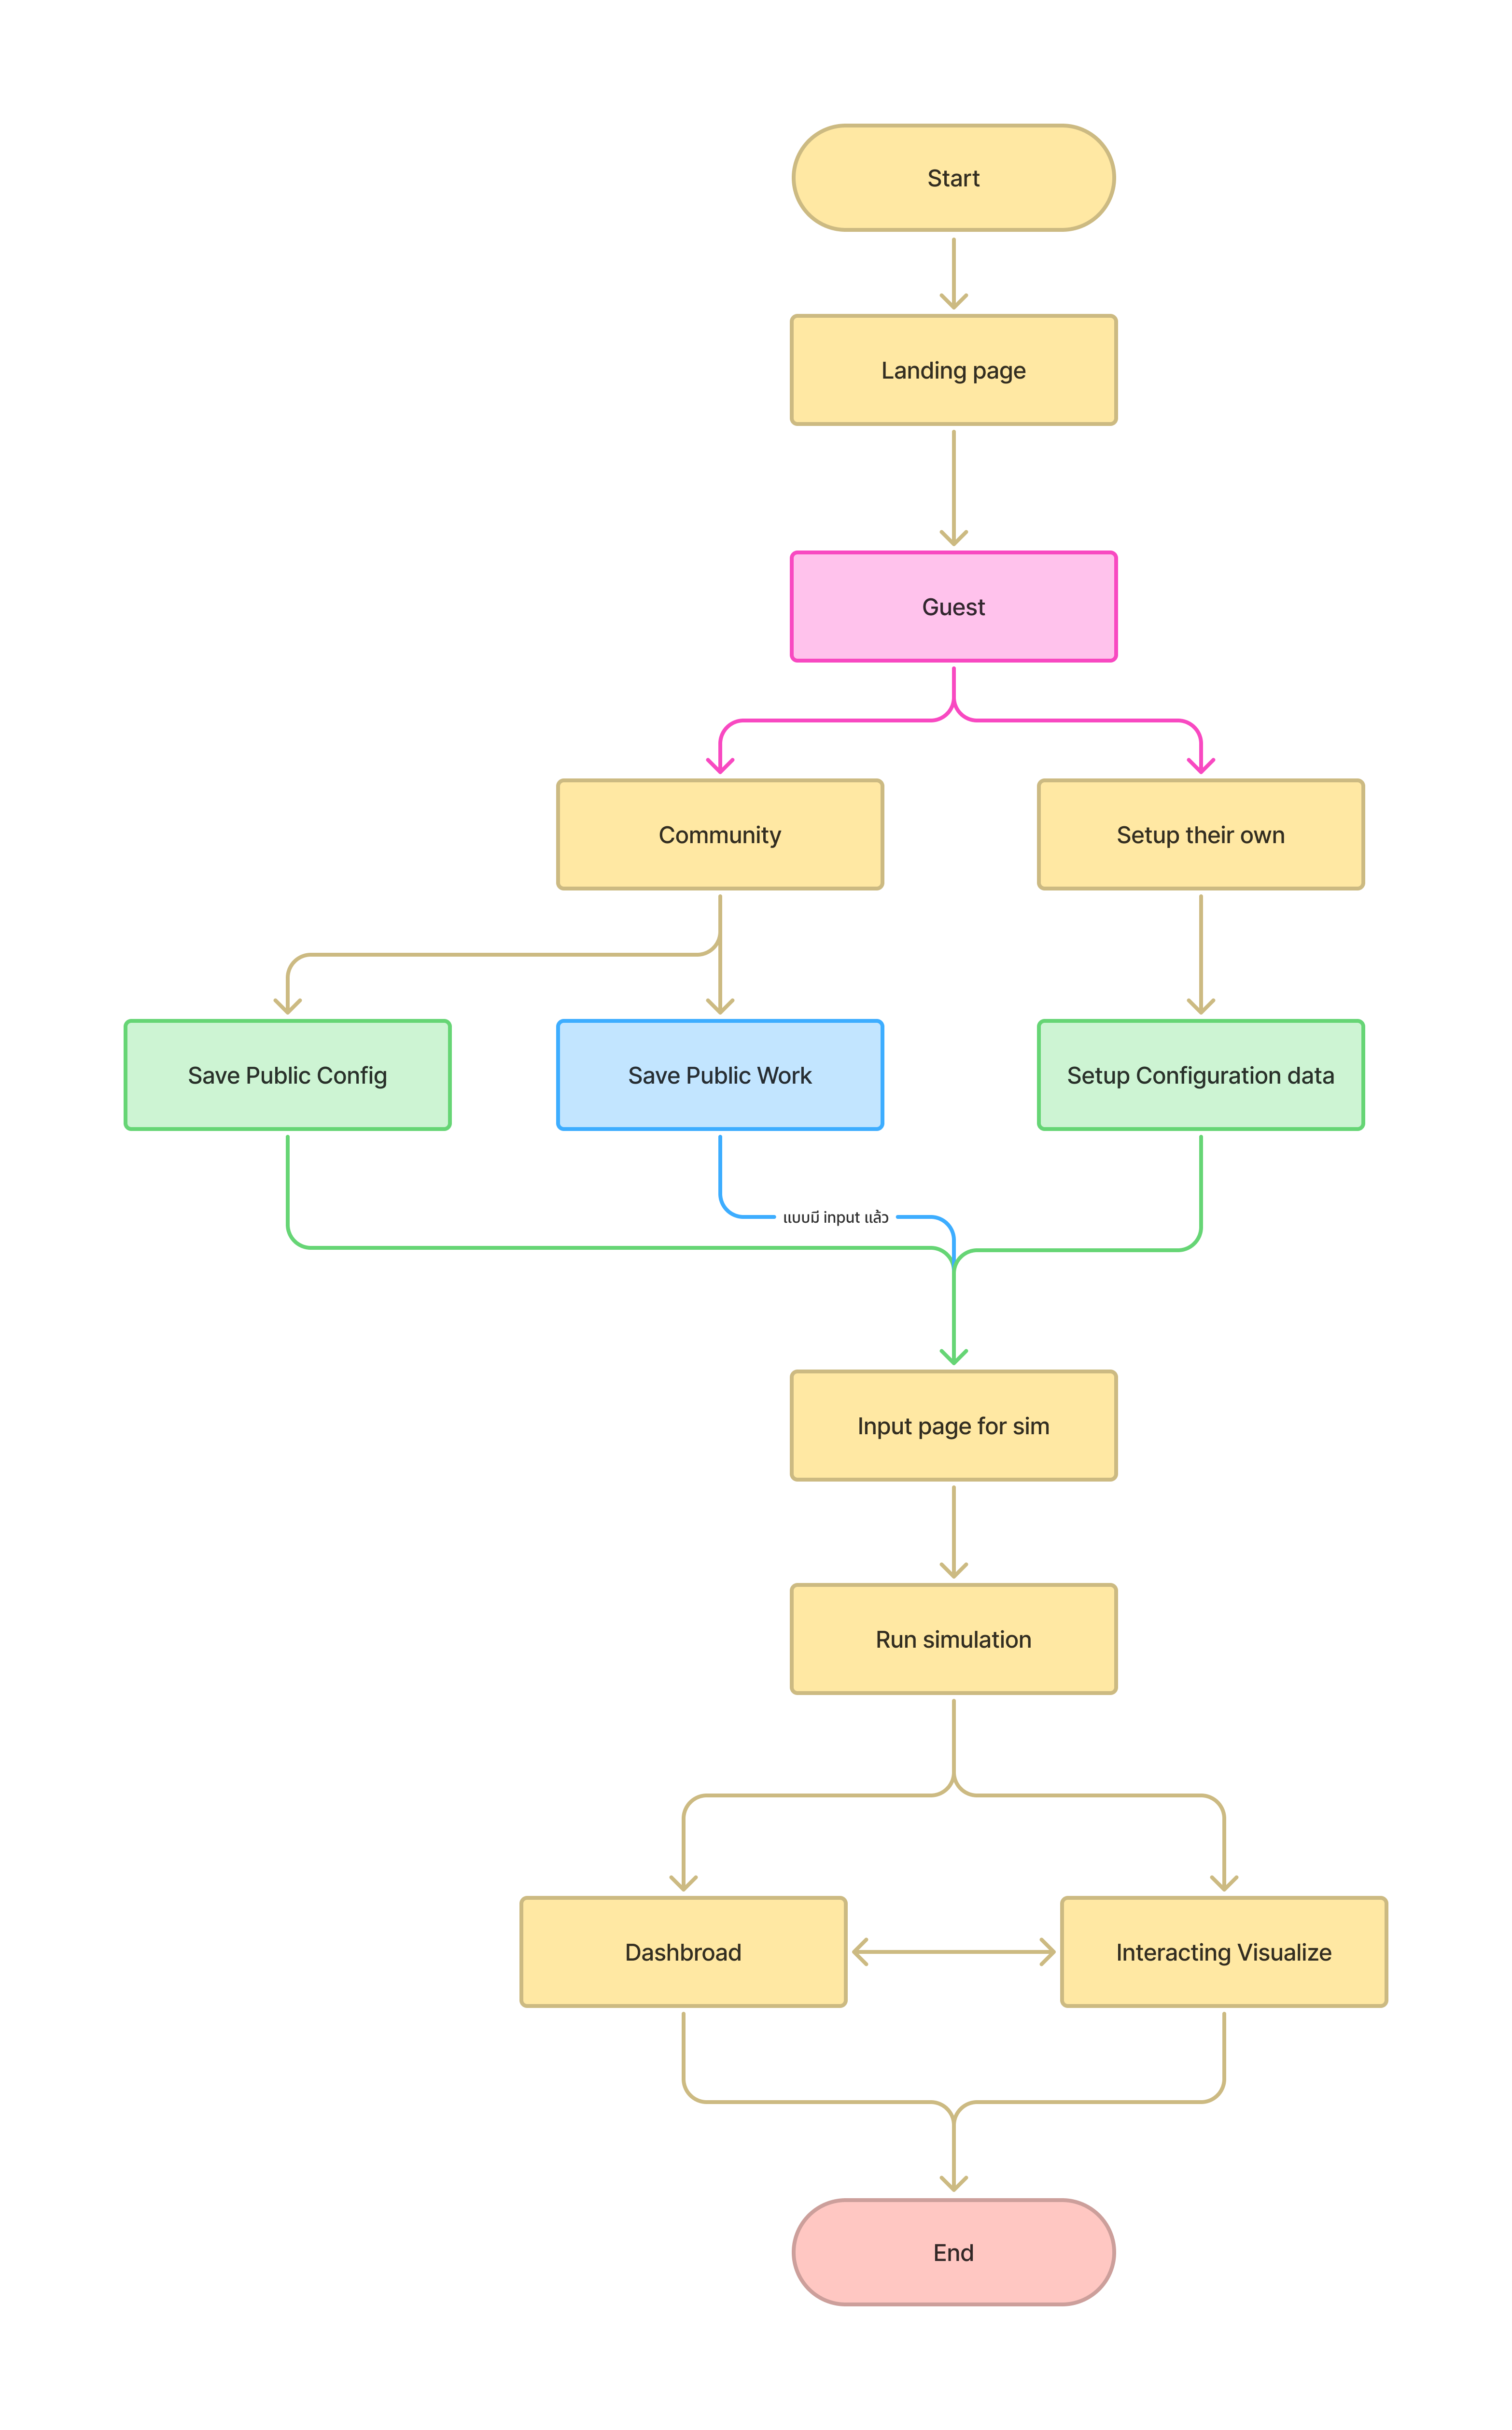
\includegraphics[width=\textwidth,height=0.6\textheight,keepaspectratio]{User_flow_-_guest.png}
      \caption{User flow  ของผู้ใช้ที่ไม่ได้ลงทะเบียน}
      \label{fig:UserFlowUnregistered}
      \end{figure}
      \newpage
      \item ผู้ใช้ที่ลงทะเบียน (Registered Users)
      \begin{figure}[H]
      \centering
      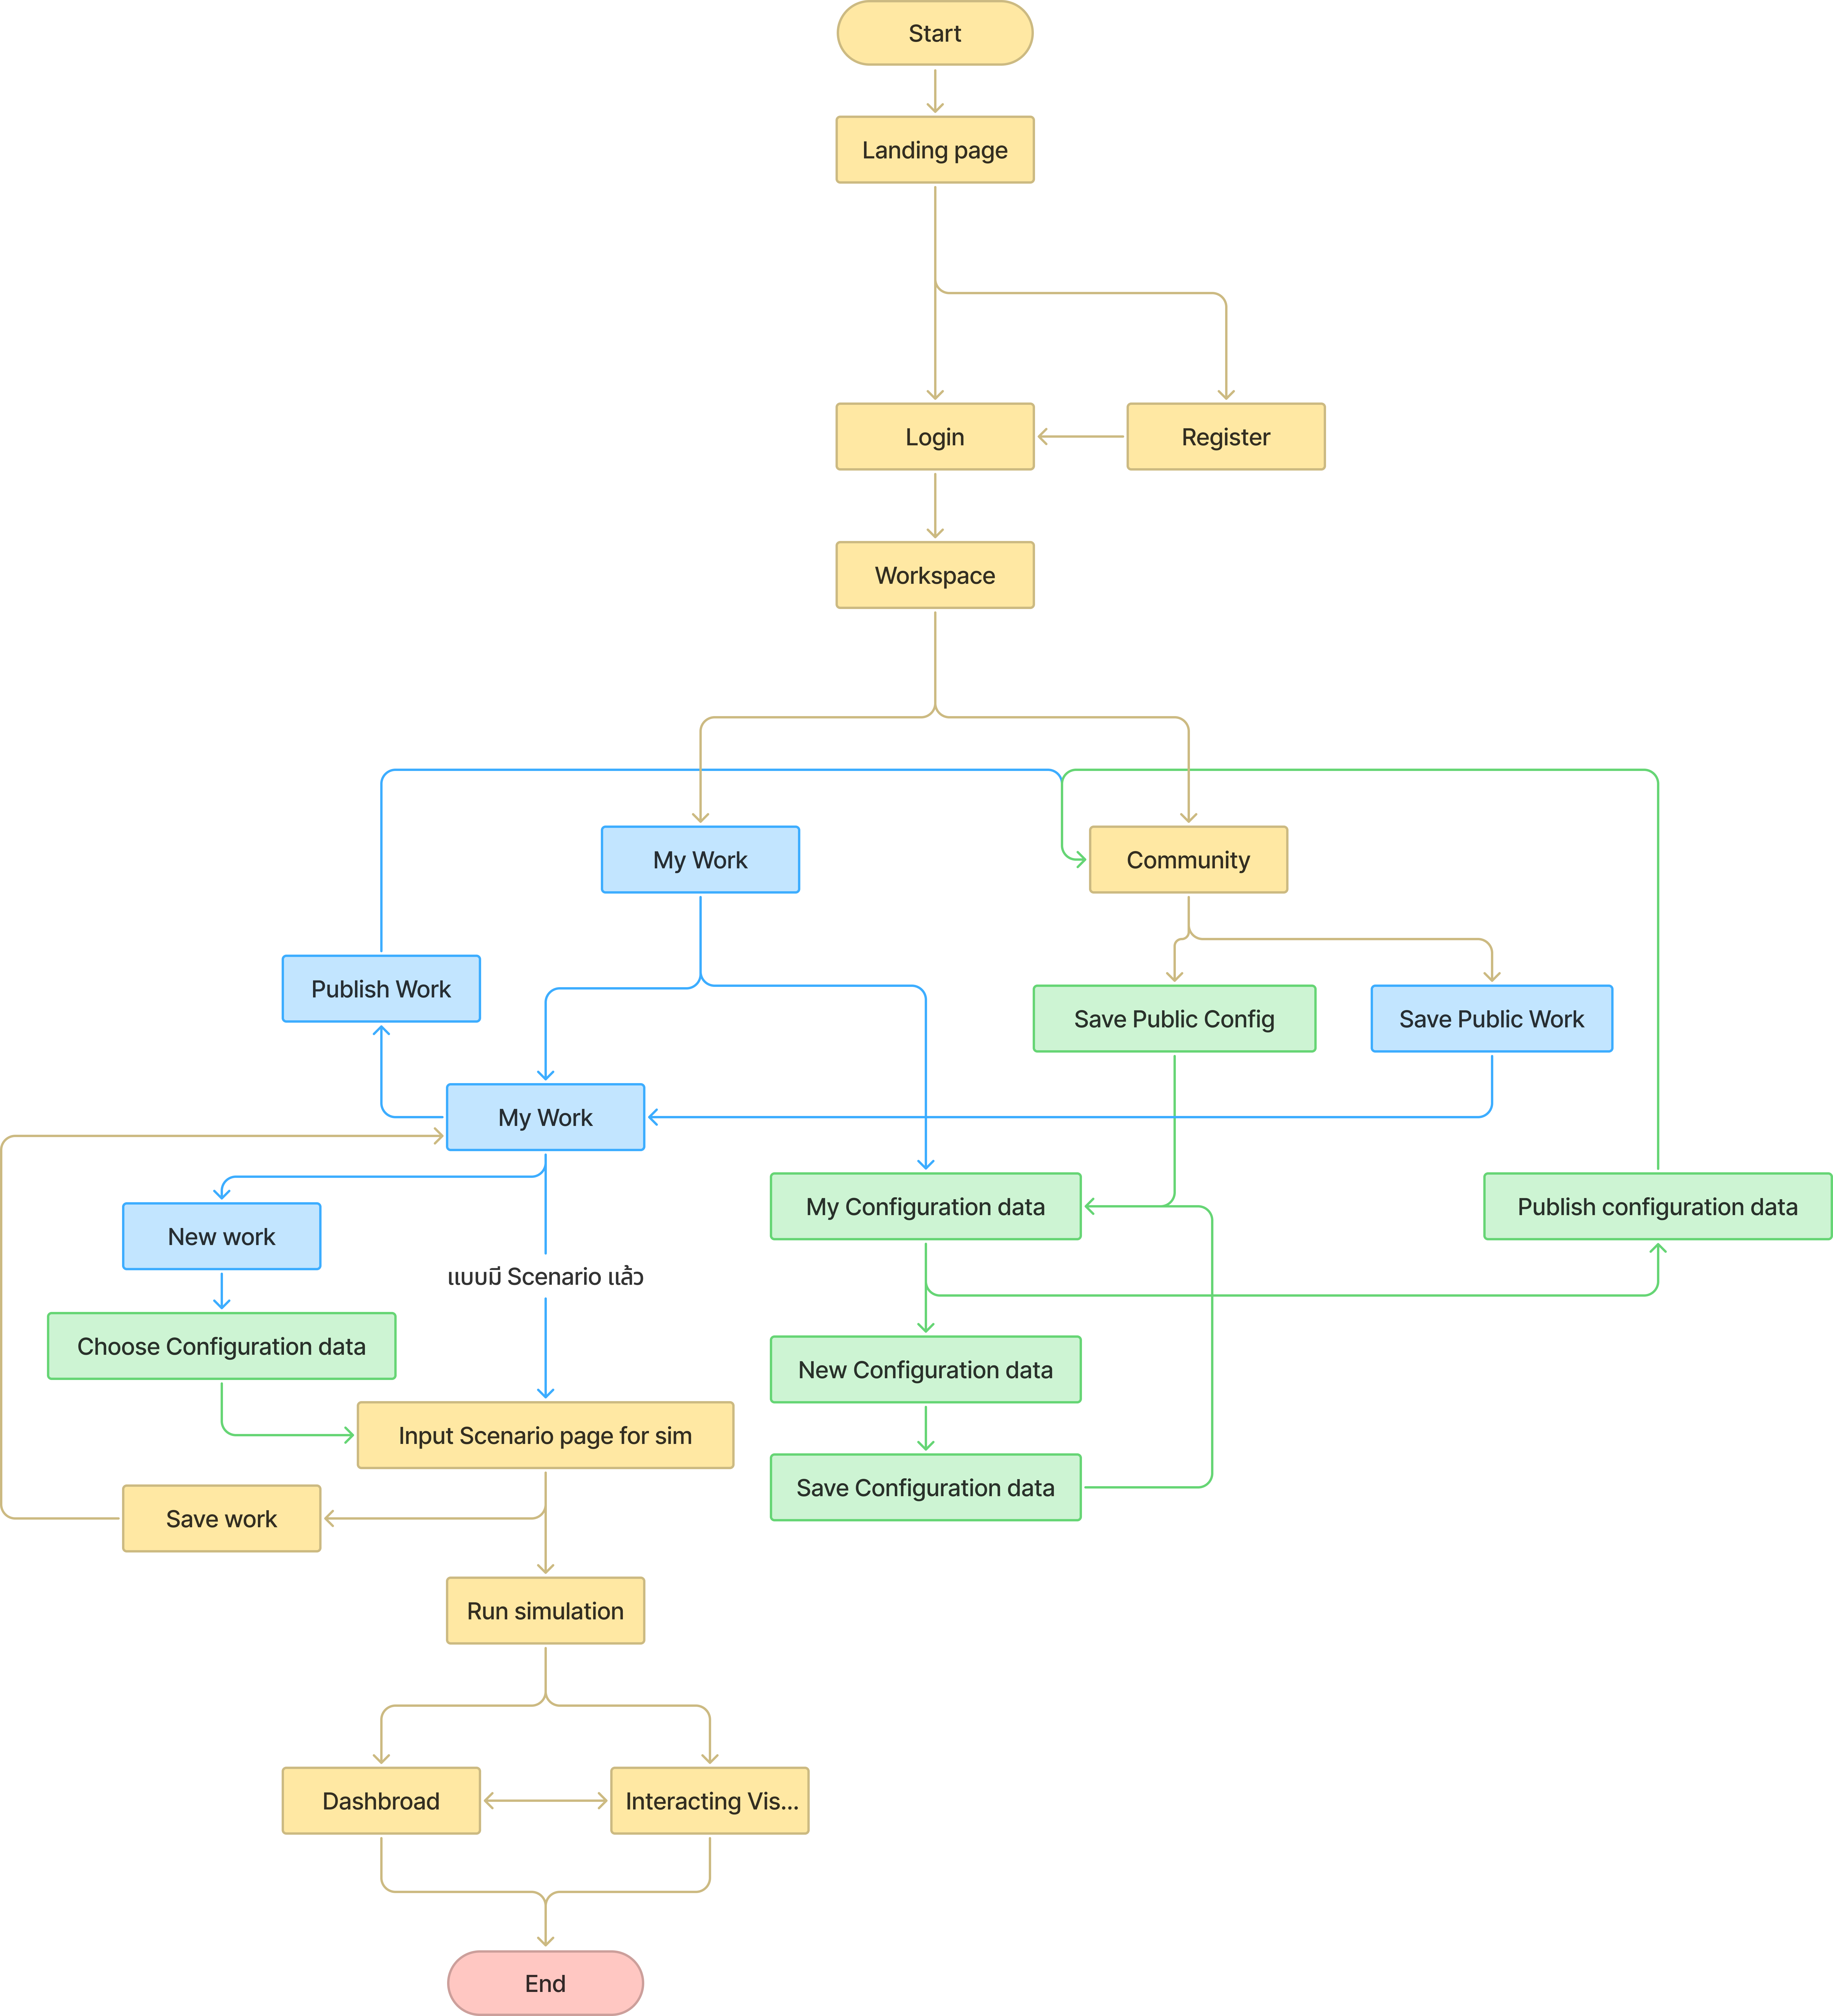
\includegraphics[width=\textwidth,height=0.9\textheight,keepaspectratio]{User_flow_-_login.png}
      \caption{User flow ของผู้ใช้ที่ลงทะเบียน}
      \label{fig:UserFlowRegistered}
      \end{figure}
      

  \end{itemize}
\newpage
\section{Wireframe}
\begin{mypara}
    \indent โครงงานนี้มีการออกแบบ Wireframe สำหรับหน้าต่างๆ ของระบบ 
    เพื่อใช้เป็นแนวทางในการพัฒนาและทดสอบระบบ โดย Wireframe ที่ออกแบบมีดังนี้

\subsection{Wireframe ผู้ใช้ที่ไม่ได้ลงทะเบียน (Guest Users / Unregistered Users)}
\begin{itemize}
    \item Step 1: ผู้ใช้จะเข้าสู่หน้า Landing page เพื่อเลือกระหว่างจะเข้าใช้ในโหมด Guest user หรือ Login user
      \begin{figure}[H]
        \centering
        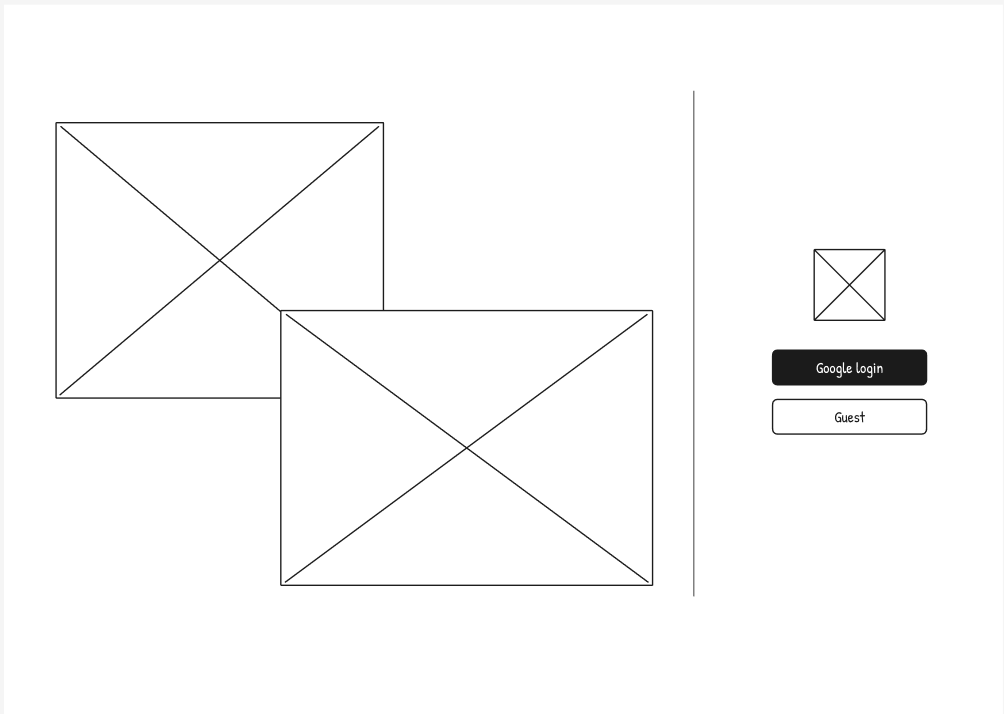
\includegraphics[scale=0.35]
        {homepage.png}
        \caption{Wireframe ของหน้า Landing page}
        \label{fig:WireframeHomepage}
      \end{figure}

    \item Step 2: Guest user สามารถเลือกว่าจะใช้ข้อมูลที่มีอยู่ใน Community หรือเลือกที่จะ Setup ข้อมูลทั้งหมดเอง
      \begin{figure}[H]
        \centering
        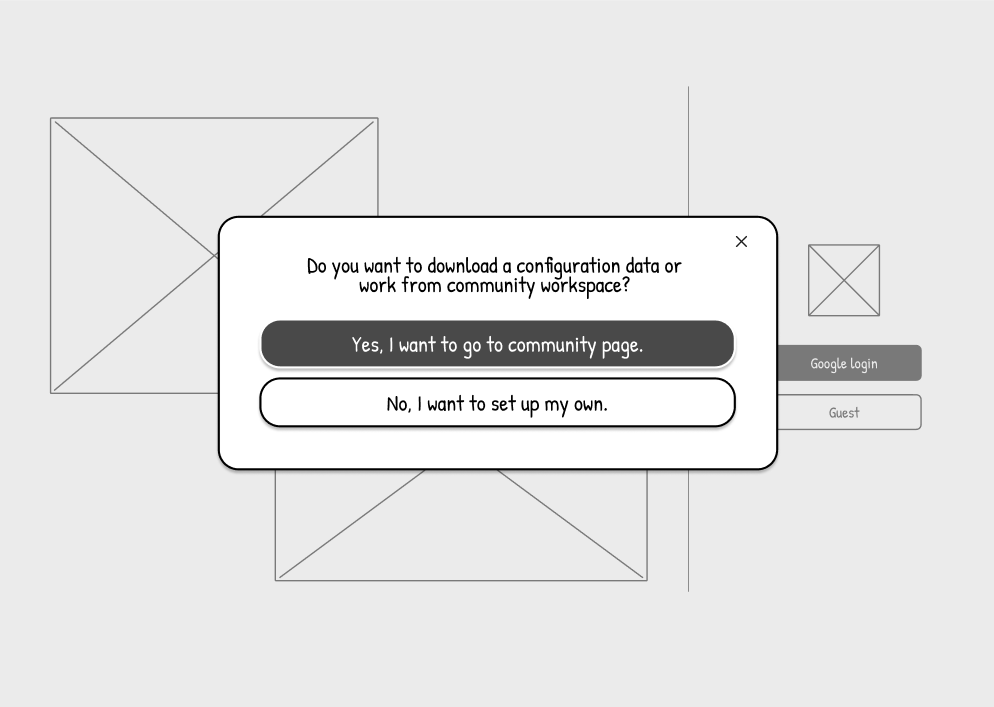
\includegraphics[scale=0.35]
        {guest_login.png}
        \caption{Wireframe ของหน้า Guest Decision}
        \label{fig:WireframeGuestDecision}
      \end{figure}

    \item Step 3: การใช้ข้อมูล Configuration data
    \begin{itemize}
        \item กรณีที่เลือกใช้จากข้อมูลที่มีอยู่ใน Community
          \begin{figure}[H]
            \centering
            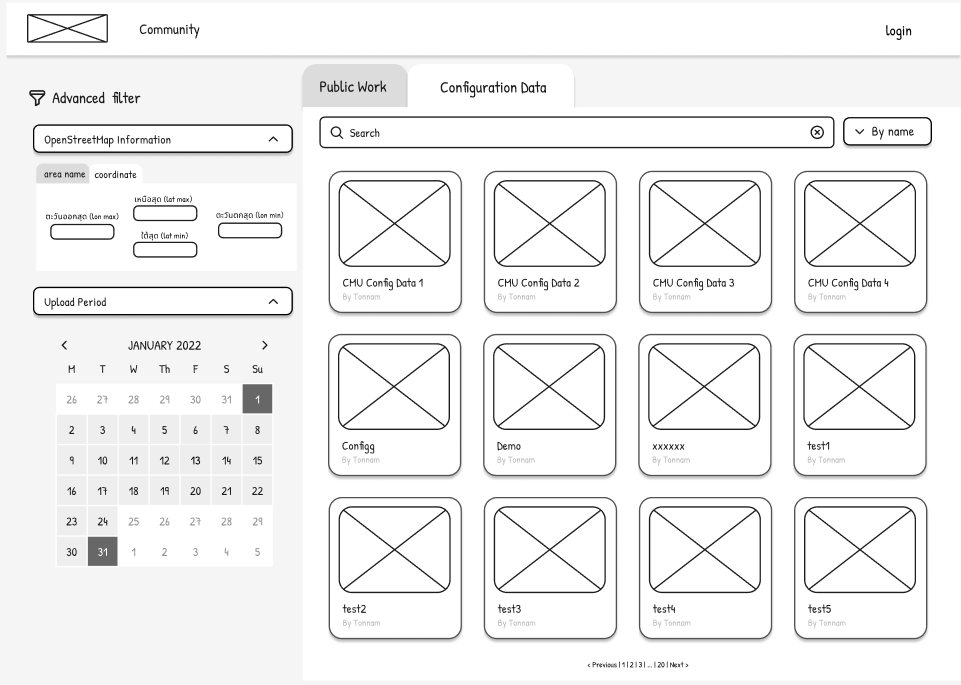
\includegraphics[scale=0.4]{conf_commu_guest.png}
            \caption{Wireframe ของหน้า Community Configuration data}
            \label{fig:WireframeCommunityConfigGuest}
          \end{figure}

          \begin{figure}[H]
            \centering
            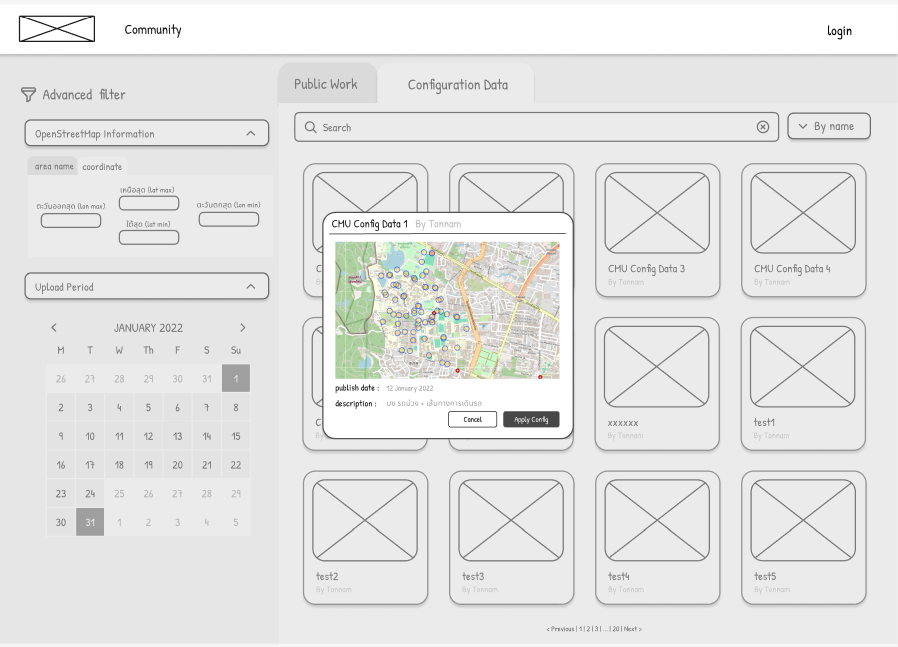
\includegraphics[scale=0.4]{conf_commu_detail_guest.png}
            \caption{Wireframe ของหน้ารายละเอียด Configuration data ใน Community}
            \label{fig:WireframeCommunityConfigDetailGuest}
          \end{figure}

        \newpage
        \item กรณีที่ผู้ใช้เลือก Setup ข้อมูลทั้งหมดเอง จะเข้าสู่การ Setup Configuration ด้วยตนเอง
          \begin{figure}[H]
            \centering
            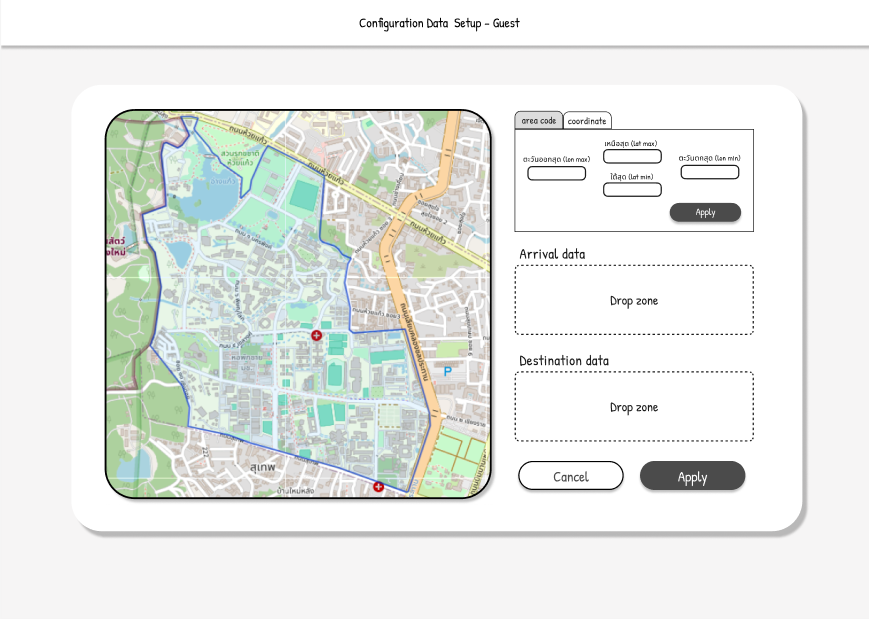
\includegraphics[scale=0.4]{conf_setup_guest.png}
            \caption{Wireframe ของหน้า Setup Configuration data สำหรับ Guest}
            \label{fig:WireframeSetupConfigGuest}
          \end{figure}
    \end{itemize}

    \item Step 4: หลังจาก Setup Configuration data ทั้งหมดเรียบร้อยจะเข้าสู่หน้า Input page เพื่อกรอกข้อมูลสำหรับการจำลองบน Scenario ต่างๆ
      \begin{figure}[H]
        \centering
        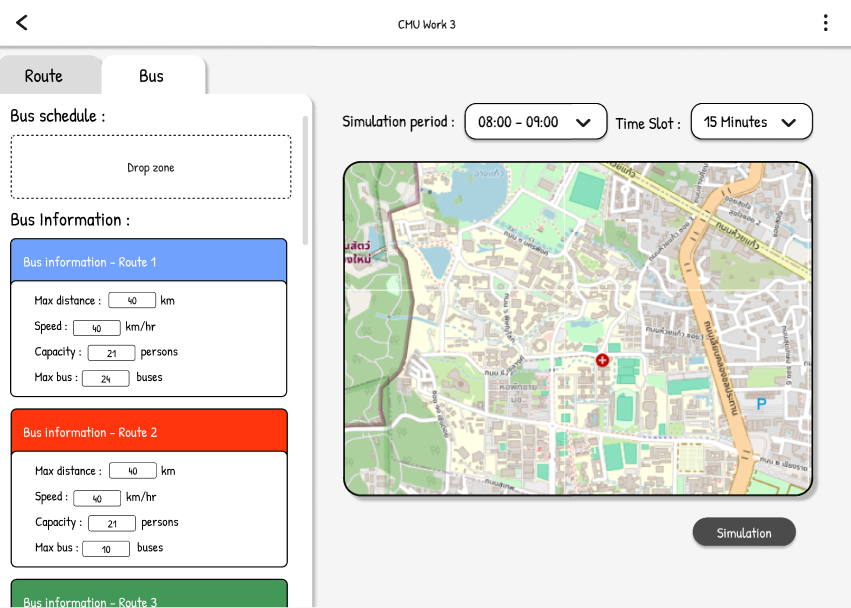
\includegraphics[scale=0.4]{input_bus.png}
        \caption{Wireframe ของหน้า Input page (bus) }
        \label{fig:WireframeInputGuest}
      \end{figure}
      \begin{figure}[H]
        \centering
        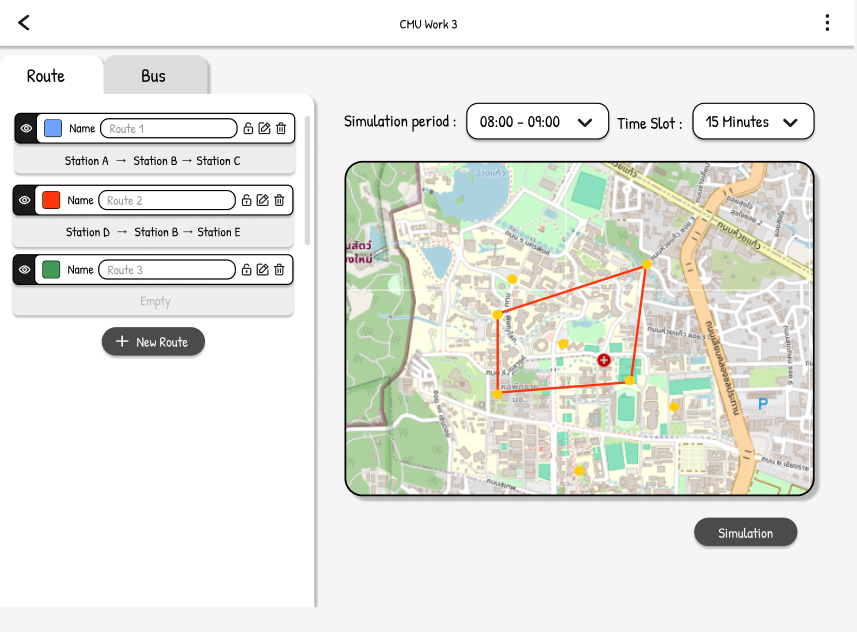
\includegraphics[scale=0.4]{input_route.png}
        \caption{Wireframe ของหน้า Input page (route) }
        \label{fig:WireframeInputRouteGuest}
      \end{figure}

    \item Step 5: หลังจากผู้ใช้กดปุ่ม Run simulation แล้ว User จะสามารถเลือกดู  Dashboard สรุปผลข้อมูล 
    หรือ Interacting Visualize
      \begin{figure}[H]
        \centering
        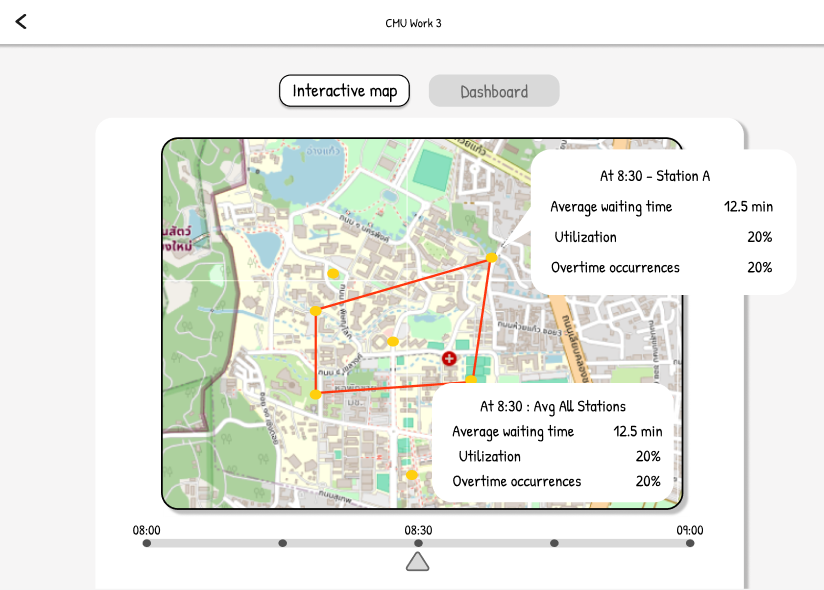
\includegraphics[scale=0.4]{output_show.png}
        \caption{Wireframe ของหน้าแสดงผลลัพธ์หลังจาก Run Simulation}
        \label{fig:WireframeOutputGuest}
      \end{figure} 

      \begin{figure}[H]
        \centering
        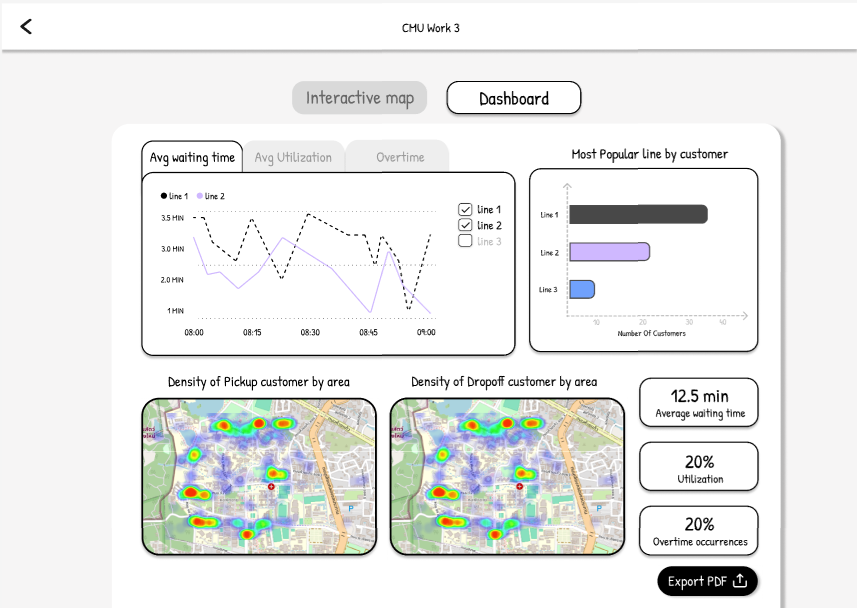
\includegraphics[scale=0.4]{dashboard.png}
        \caption{Wireframe ของหน้า Dashboard }
        \label{fig:WireframeDashboardGuest}
      \end{figure}
    
\end{itemize} 


\subsection{Wireframe ของผู้ใช้ที่ลงทะเบียน (Registered Users)}
\begin{itemize}
    \item Step 1:  ผู้ใช้จะเข้าสู่หน้า Landing page เพื่อเลือกระหว่างจะเข้าใช้ในโหมด Guest user หรือ Login user
    \begin{figure}[H]
    \centering
    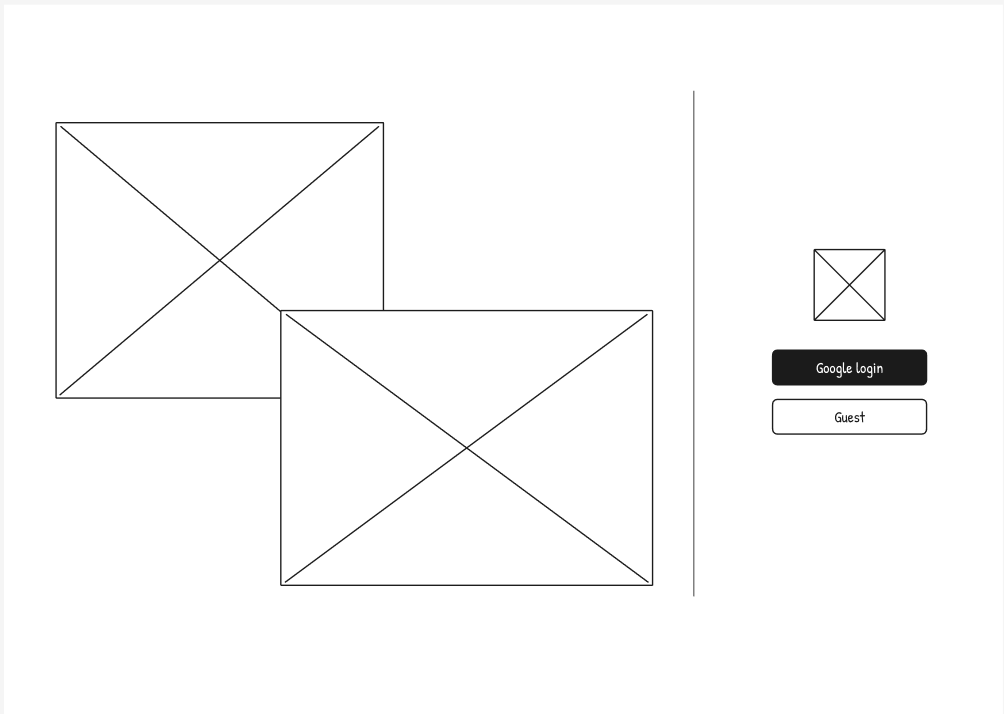
\includegraphics[scale=0.4]
    {homepage.png}
    \caption{Wireframe ของหน้า Landing page}
    \label{fig:WireframeHomepageLogin}
    \end{figure}

    \newpage
    \item Step 2: หลังจากเข้าสู่ระบบผู้ใช้จะเข้าสู่หน้า My work ซึ่งเป็นการจัดการงานทั้งหมดของผู้ใช้
    \begin{itemize}
      \item ในหน้า My work ผู้ใช้สามารถเลือกใช้งานหรือ Publish งาน
        \begin{figure}[H]
          \centering
          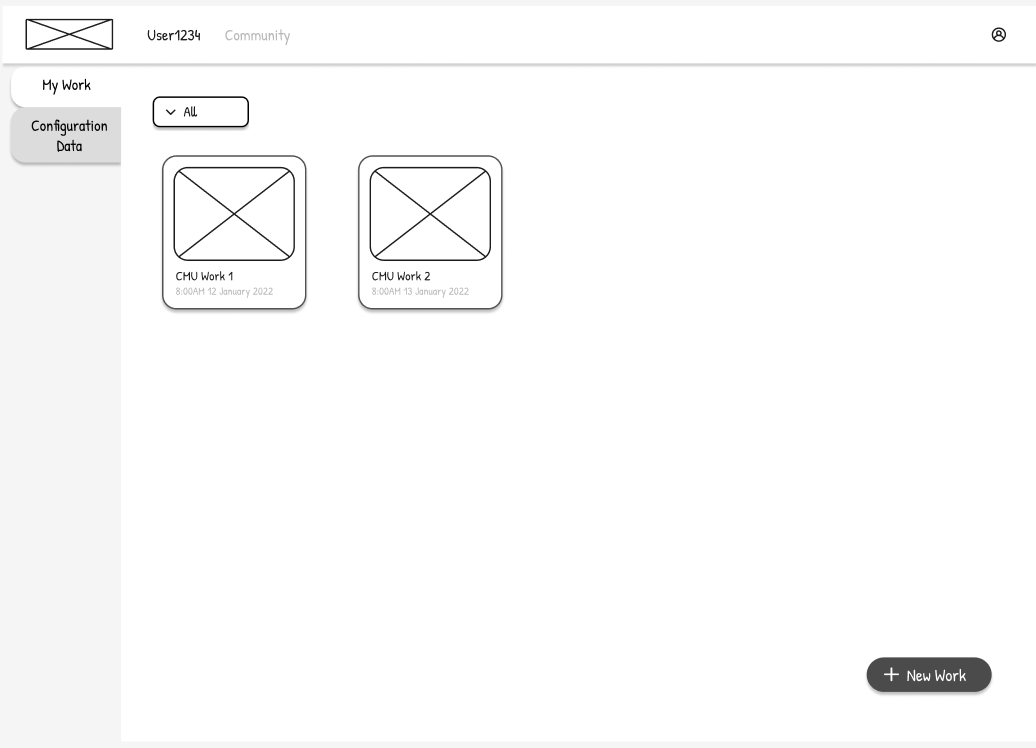
\includegraphics[scale=0.4]{my_work.png} 
          \caption{Wireframe ของหน้า My work}
          \label{fig:WireframeMyWork}
        \end{figure}

        \begin{figure}[H]
          \centering
          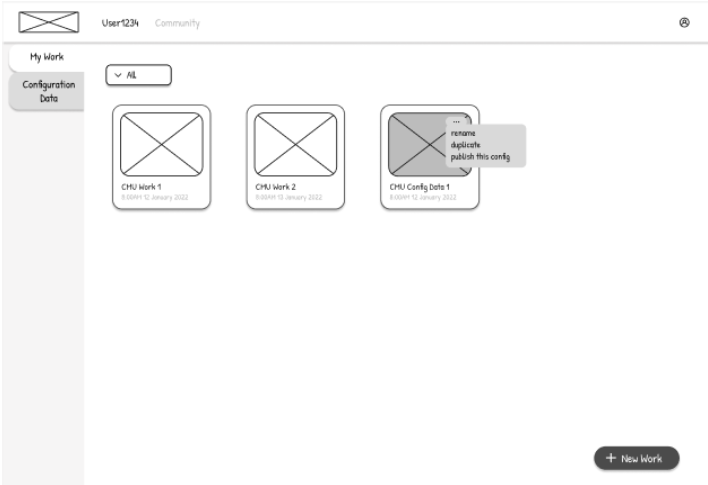
\includegraphics[scale=0.6]{my_work_publish.png} 
          \caption{Wireframe ของหน้า My work ในกรณีที่ Publish งาน}
          \label{fig:WireframeMyWorkPublish}
        \end{figure}
        
      \newpage
      \item  ผู้ใช้สามารถสร้าง Work ใหม่ได้ด้วยการกดที่ปุ่ม New work โดยการสร้าง Work จะต้องอ้างอิงกับ Configuration data ที่มีอยู่
        \begin{figure}[H]
        \centering
        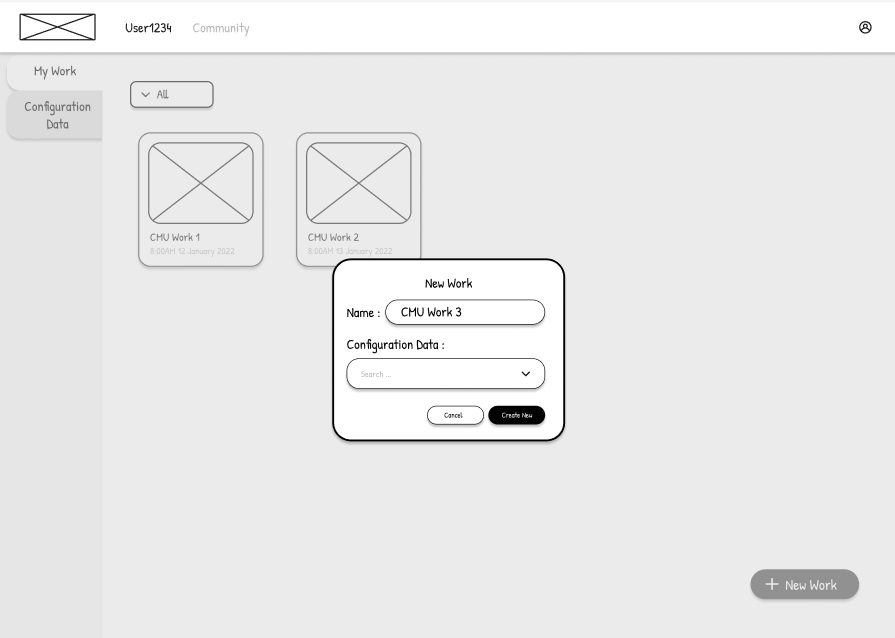
\includegraphics[scale=0.4]{new_work.png}
        \caption{Wireframe ของหน้า New work}
        \label{fig:WireframeNewWork}
        \end{figure}
    \end{itemize}

    \item Step 3: การใช้ข้อมูล Configuration data
    \begin{itemize}
        \item กรณีที่เลือกใช้จากข้อมูลที่มีอยู่ใน Community
          \begin{figure}[H]
            \centering
            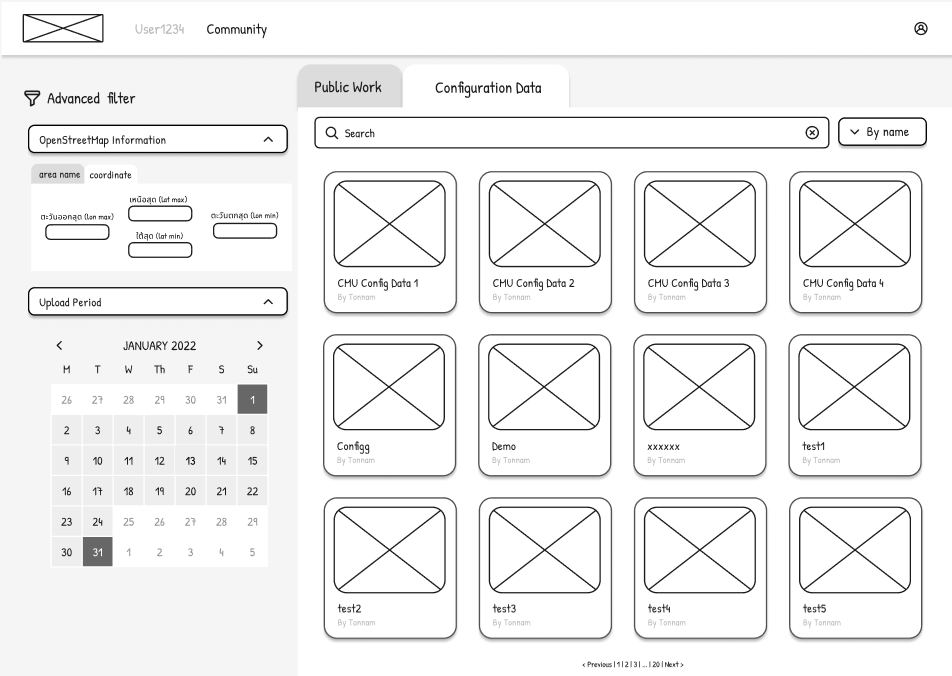
\includegraphics[scale=0.4]{conf_commu.png}
            \caption{Wireframe ของหน้า Community Configuration data}
            \label{fig:WireframeCommunityConfigLogin}
          \end{figure}

          \begin{figure}[H]
            \centering
            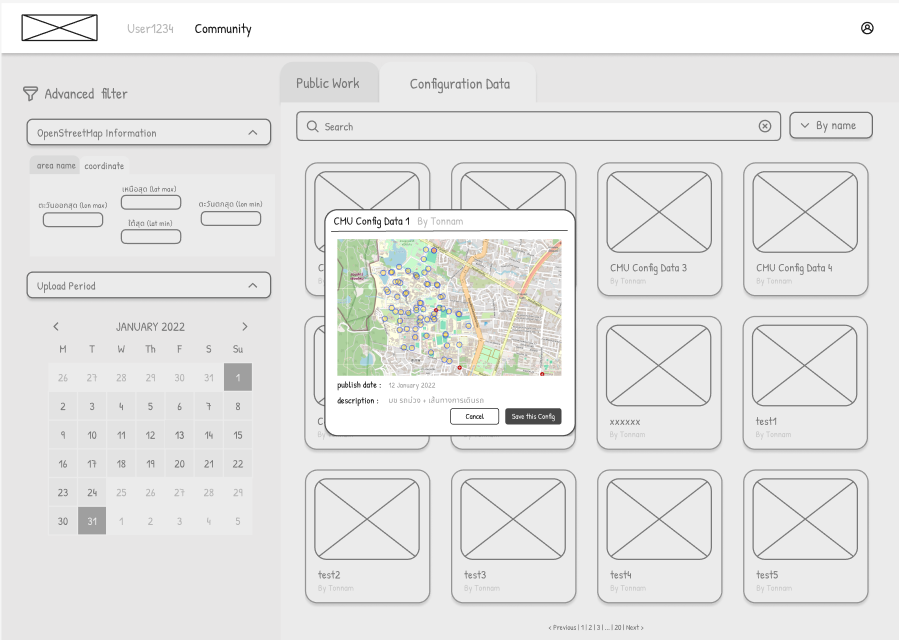
\includegraphics[scale=0.4]{conf_commu_detail_reg.png}
            \caption{Wireframe ของหน้ารายละเอียด Configuration data ใน Community}
            \label{fig:WireframeCommunityConfigDetailLogin}
          \end{figure}

        \item ผู้ใช้สามารถสร้าง Configuration data ใหม่ได้ด้วยการกดที่ปุ่ม New Configuration และสามารถ Save Configuration เพื่อใช้ในงานต่อไปได้
          \begin{figure}[H]
            \centering
            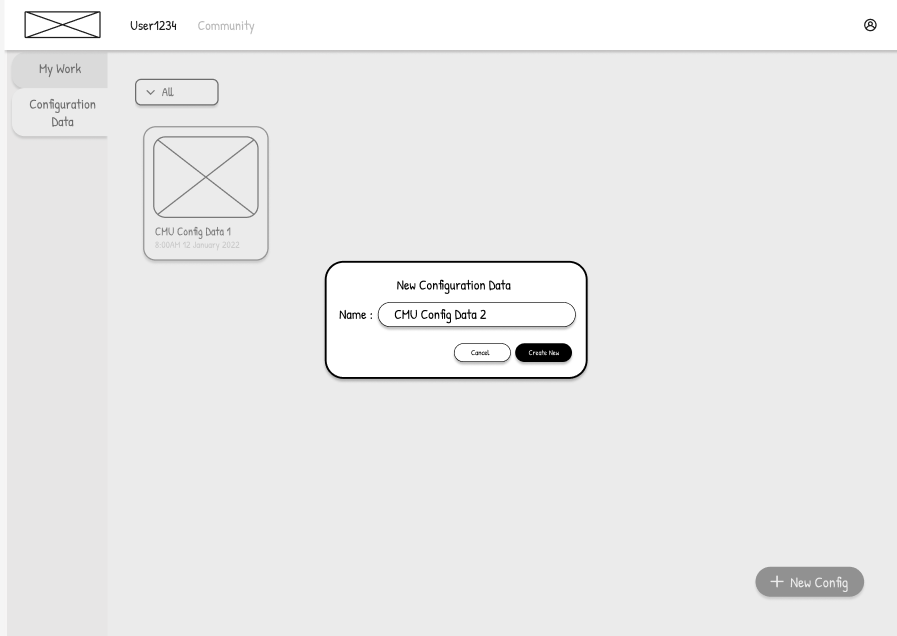
\includegraphics[scale=0.4]{new_conf.png}
            \caption{Wireframe ของหน้า New Configuration data}
            \label{fig:WireframeNewConfigLogin}
          \end{figure}

          \begin{figure}[H]
            \centering
            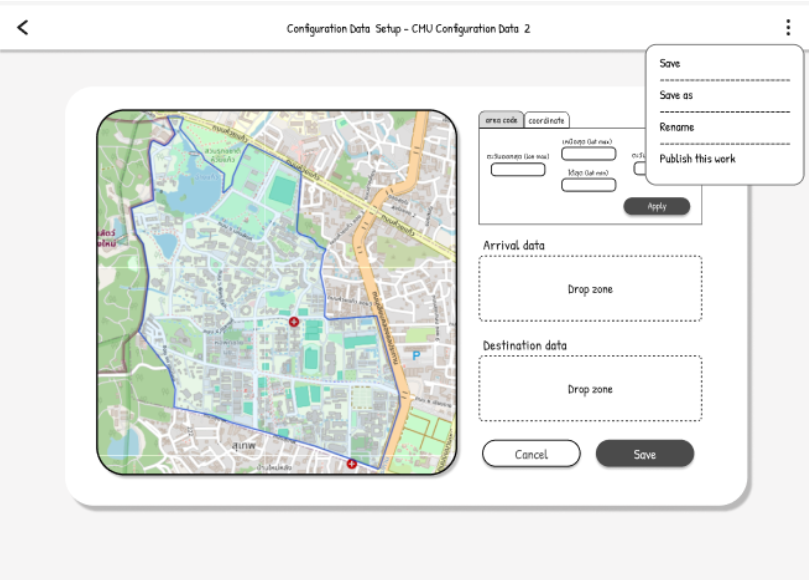
\includegraphics[scale=0.4]{conf_setup_reg.png}
            \caption{Wireframe ของหน้า Setup Configuration data สำหรับผู้ใช้ที่ลงทะเบียน}
            \label{fig:WireframeSetupConfigLogin}
          \end{figure}

    \end{itemize}

    \item Step 4: หน้า Input page เพื่อกรอกข้อมูลสำหรับการจำลองบน Scenario ต่างๆ
      \begin{figure}[H]
        \centering 
        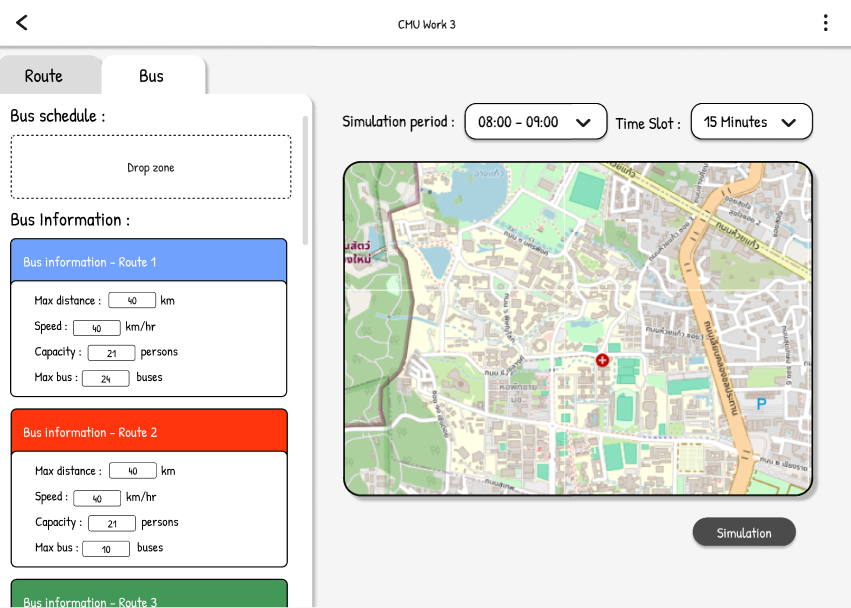
\includegraphics[scale=0.4]{input_bus.png}
        \caption{Wireframe ของหน้า Input page (bus) }
        \label{fig:WireframeInputLogin}
      \end{figure}

      \begin{figure}[H]
        \centering
        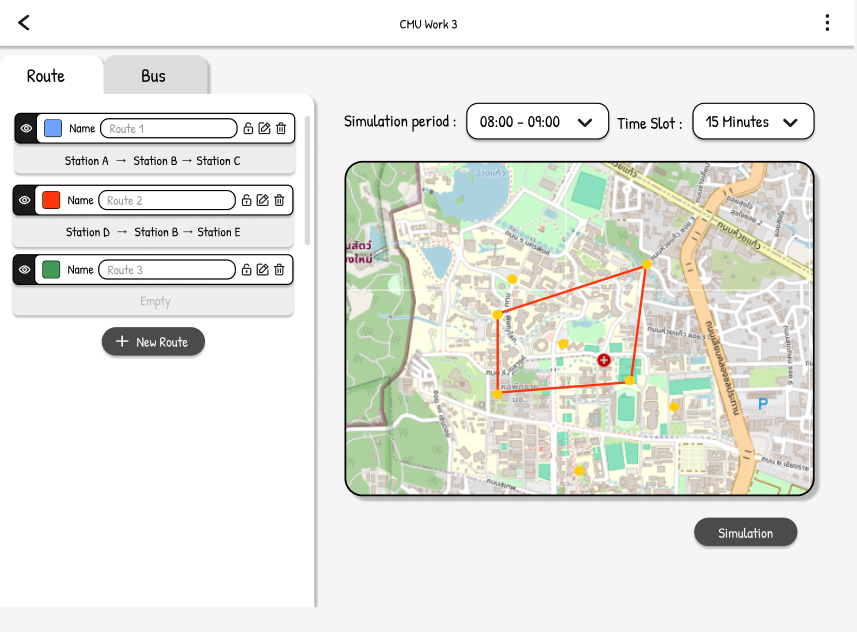
\includegraphics[scale=0.4]{input_route.png}
        \caption{Wireframe ของหน้า Input page (route) }
        \label{fig:WireframeInputRouteLogin}
      \end{figure}

    \item Step 5: หลังจากผู้ใช้กดปุ่ม Run simulation แล้ว User จะสามารถเลือกดู  Dashboard สรุปผลข้อมูล 
      \begin{figure}[H]
        \centering
        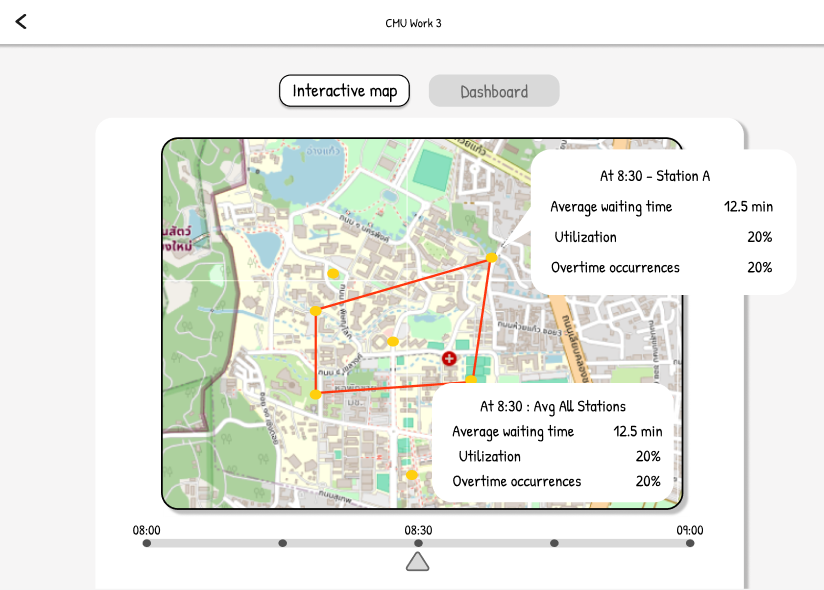
\includegraphics[scale=0.4]{output_show.png}
        \caption{Wireframe ของหน้าแสดงผลลัพธ์หลังจาก Run simulation}
        \label{fig:WireframeOutputLogin}
      \end{figure}

      \begin{figure}[H]
        \centering
        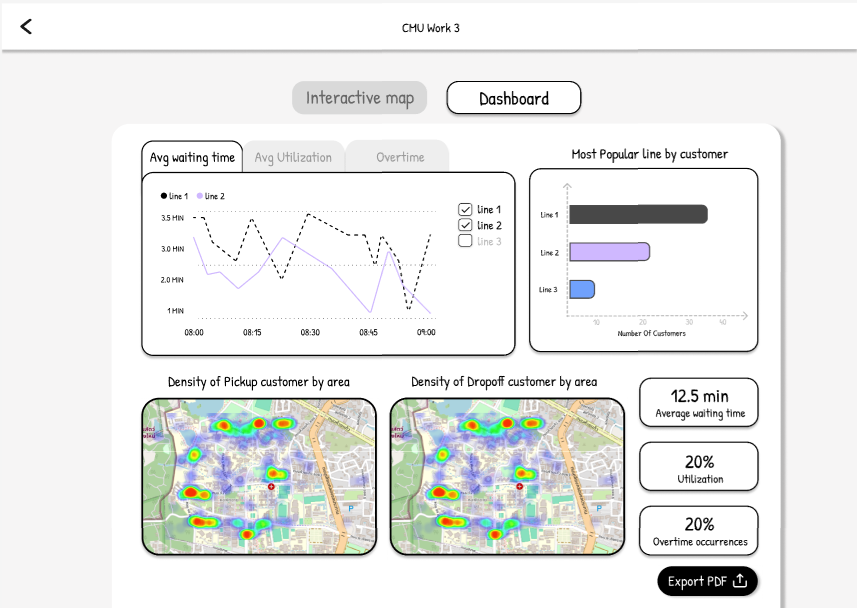
\includegraphics[scale=0.4]{dashboard.png}
        \caption{Wireframe ของหน้า Dashboard }
        \label{fig:WireframeDashboardLogin}
      \end{figure}
    \end{itemize}

\end{mypara}

\section{รูปแบบไฟล์ข้อมูลนำเข้า (Supported Input File Formats)}
  \subsection{รูปแบบไฟล์ช่วงเวลาในการมาถึงของผู้โดยสาร (Passenger Arrival Time File Format)}
  \begin{mypara}
      \indent รูปแบบไฟล์ช่วงเวลาในการมาถึงของผู้โดยสาร ใช้สำหรับเก็บข้อมูลช่วงเวลาที่ผู้โดยสารแต่ละคนมาถึงที่สถานี
      โดยข้อมูลจะถูกจัดเก็บในไฟล์ Excel โดยมีสกุลไฟล์ \texttt{.xlsx} 
      ซึ่งมีโครงสร้างดังแสดงในภาพด้านล่าง
      \begin{figure}[H]
        \centering
        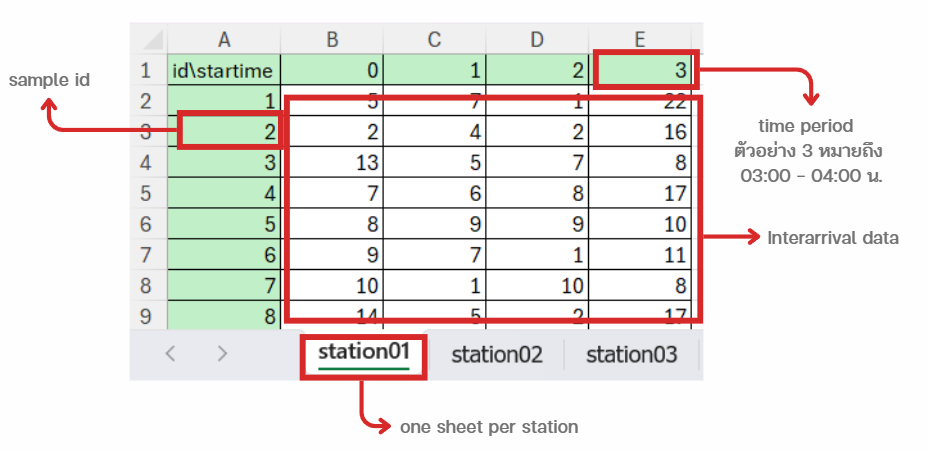
\includegraphics[scale=0.5]{Passenger_Interarrival.png}
        \caption{รูปแบบไฟล์ช่วงเวลาในการมาถึงของผู้โดยสาร}
        \label{fig:PassengerArrivalFileFormat}
      \end{figure}
  \end{mypara}

  \newpage
  \subsection{รูปแบบไฟล์จำนวนผู้โดยสารที่ลงจากรถ (Passenger Alight File Format)}
  \begin{mypara}
      \indent รูปแบบไฟล์จำนวนผู้โดยสารที่ลงจากรถ ใช้สำหรับเก็บข้อมูลจำนวนผู้โดยสารที่ลงจากรถในแต่ละสถานี
      โดยข้อมูลจะถูกจัดเก็บในไฟล์ Excel โดยมีสกุลไฟล์ \texttt{.xlsx} 
      ซึ่งมีโครงสร้างดังแสดงในภาพด้านล่าง
      \begin{figure}[H]
        \centering
        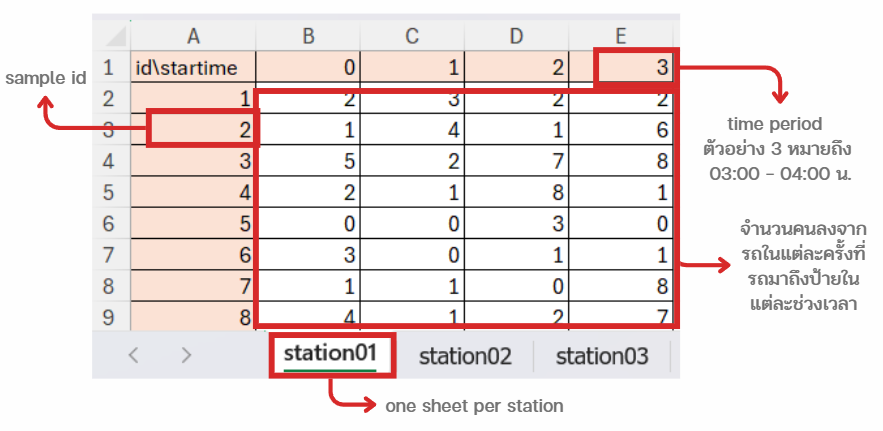
\includegraphics[scale=0.5]{Passenger_alighting.png}
        \caption{รูปแบบไฟล์จำนวนผู้โดยสารที่ลงจากรถ}
        \label{fig:PassengerAlightFileFormat}
      \end{figure}
  \end{mypara}

  \subsection{รูปแบบไฟล์ตารางการเดินรถ (Bus Schedule File Format)}
  \begin{mypara}
      \indent รูปแบบไฟล์ตารางการเดินรถ ใช้สำหรับเก็บข้อมูลเวลาการออกรถของแต่ละสายบริการ 
      โดยข้อมูลจะถูกจัดเก็บในไฟล์ Excel โดยมีสกุลไฟล์ \texttt{.xlsx} 
      ซึ่งมีโครงสร้างดังแสดงในภาพด้านล่าง
      \begin{figure}[H]
        \centering
        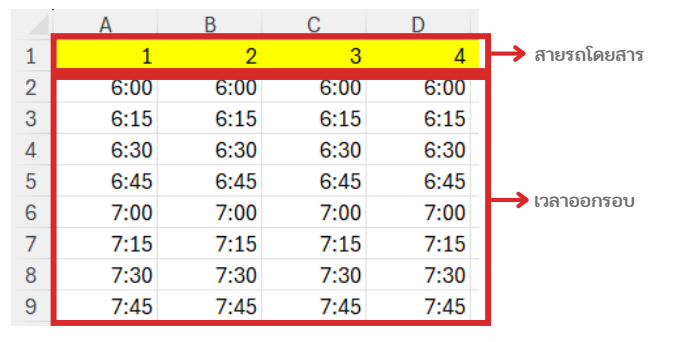
\includegraphics[scale=0.5]{bus_schedule.png}
        \caption{รูปแบบไฟล์ตารางการเดินรถ}
        \label{fig:BusScheduleFileFormat}
      \end{figure}
  \end{mypara}